\label{sec:muroexe}

MuroEXE's design philosophy is to use CNN as much as possible to accomplish various tasks of the robot. Because the CNN not only has advantages over traditional algorithms in accuracy, but also has uniform and regular computing mode. Therefore, a single instruction-driven CNN accelerator can speed up different tasks. The unified accelerator can reduce the use of hardware resources and reduce the difficulty of system development.



\begin{figure}[t]
	\centering
    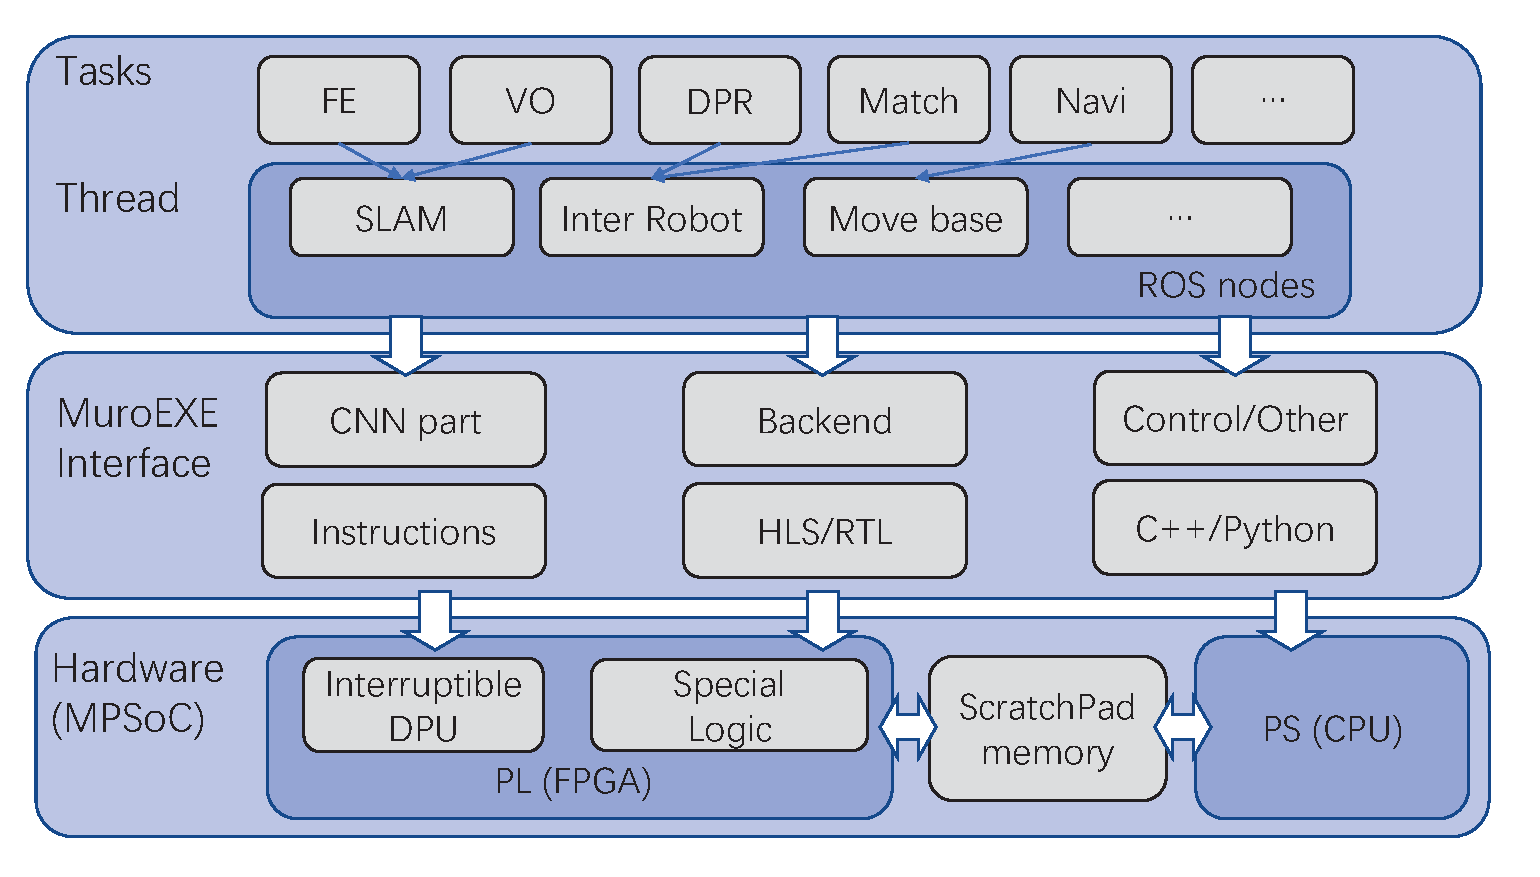
\includegraphics[width=0.99\linewidth]{fig/muroexe.eps}
    \caption{ Overview of the MUROEXE framework. Each ROS node is a separate thread. The CNNs in differetn ROS nodes are deployed onto the interruptible accelerator. The post-processing in the ROS nodes can accelerated by the RTL/HLS modules. The hardware modules for post-processing and the CNN accelerator share data through scrachpad memory. }
	\label{fig:muroexe}
\end{figure}